\chapter{مقدمه}
پویانمایی هنر جان‌بخشیدن به اجسام بدون جان است.

والت دیزنی درباره‌‌ی پویانمایی می‌گوید: "انیمیشن می تواند هر آنچه را که ذهن انسان تصور می کند توضیح دهد"
وقتی می‌گوییم جسمی را پویا کردیم، یعنی به آن جان بخشیدیم.
زمانی که یک فیلم پویانمایی شده را در تلوزیون یا سینما می‌بینید، شخصیت‌های درون آن فیلم در حالت حرکت هستند.
این حرکت معمولا صاف و به هم پیوسته است. نوارهای حاوی فیلم متشکل از دنباله‌ای از تصاویر هستند که به عنوان "فریم" شناخته می‌شوند و درواقع با پخش شدن این فریم‌ها
به صورت متوالی، توهم ایجاد حرکت به مخاطب القا می‌شود.

پویانمایی تاریخچه‌ای غنی‌ دارد. در این فصل ابتدا به بررسی این تاریخچه با توضیحاتی 
درباره‌ی پویانمایی سنتی و پس از آن پویانمایی کامپیوتری پرداخته می‌شود.
پس از آن به بررسی روش‌های کلی که توسط هنرمندان برای ایجاد پویانمایی به‌کارگرفته می‌شوند پرداخته می‌شود.
در نهایت به بررسی به کارگرفتن این انیمیشن‌ها در موتورهای بازی سازی پرداخته می‌شود.

\section{تاریخچه‌ی پویانمایی سنتی}

پویانمایی سنتی که با اسم‌های مختلفی مانند "پویانمایی مرسوم" ، "پویانمایی سل‌ای"و "پویانمایی بادست" شناخته می‌شود، روشی 
غالب برای تولید فیلم‌های پویانمایی‌شده در حدود قرن 20 میلادی بود.
در این روش، به صورت کلی پویانمایی به وسیله‌ی نقاشی با دست به وجود می‌‌آمد.
درواقع هر فریم از فیلم، یک عکسی از نقاشی بود.
برای به وجود آوردن توهم حرکت، هر نقاشی اندکی با نقاشی قبلی خود تفاوت داشت.

برای تولید پویانمایی سنتی، از روش‌های مختلفی استفاده می‌شد. در اینجا به بررسی
سه عدد از این روش‌ها می‌پردازیم.

\subsection{فریم‌های کلیدی و درمیان}
از آنجایی که تولید پویایی با دست و کشیدن نقاشی کار بسیار طولانی‌ای بود، برای اینکه وقت پویانمای‌های ارشد 
ذخیره شود، این پویانماها فریم‌های اصلی یک حرکت را بر روی کاغذ ترسیم می‌کردند و 
فریم‌های میانی را پویانماهای جوان پر می‌کردند.

\begin{figure}[ht]
	\centerline{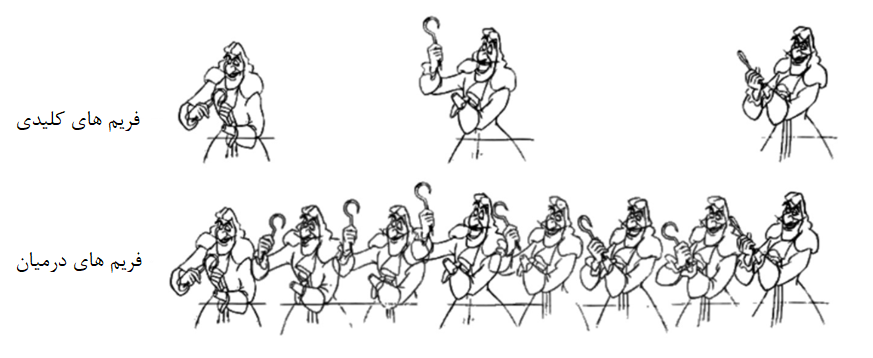
\includegraphics[width=\textwidth,height=\textheight,keepaspectratio]{Figures/Ch1/KeyframeAnimation.png}}

	\caption{فریم‌های کلیدی و درمیان}
	\label{fig:KeyframeAnimation}
\end{figure}

\subsection{چشم‌انداز چندمنظوره}

استفاده از چشم‌انداز چندمنظوره روش دیگری بود که در پویانمایی سنتی استفاده می‌شد.
هماطور که از تصویر زیر مشخص است، برای نمایش یک محیط از یک چشم‌انداز استفاده می‌شد.
این چشم‌انداز می‌توانست نشان دهنده‌ی محیط در فواصل مختلف باشد. در این صورت، زمانی که 
دوربین در صحنه حرکت می‌کرد این توهم را در مخاطب ایجاد می‌کرد که گویی در محیط در حال حرکت هستیم.

\begin{figure}[ht]
	\centerline{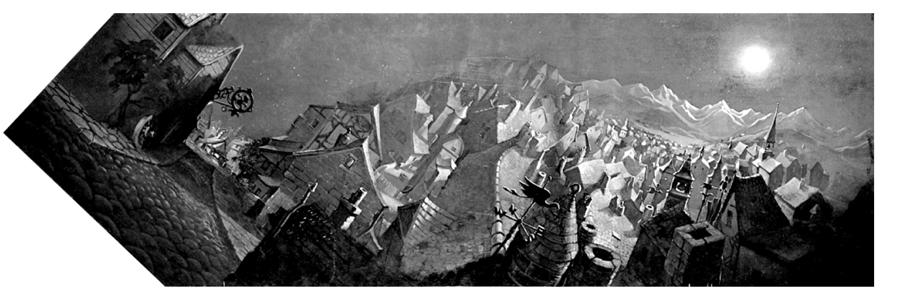
\includegraphics[width=\textwidth,height=\textheight,keepaspectratio]{Figures/Ch1/Panorama.png}}

	\caption{چشم‌انداز چندمنظوره}
	\label{fig:Panorama}
\end{figure}


\subsection{لایه‌های مختلف}

با استفاده از این روش، پویانما‌ها یک صحنه را به چند قسمت مختلف تقسیم می‌کردند.
به صورت مثال لایه‌های مختلف برای هر شخصیت درون صحنه استفاده می‌شد. علاوه برا ین یک لایه نیز برای تصویر پس‌زمینه استفاده می‌شد.
از آنجایی که این لایه‌ها یک صفحه‌ی شفاف بودند بنابراین می‌توان لایه‌‌ها را 
بر روی هم انباشته کرد و با تصویر برداری از بالا تمام صحنه را تصویربرداری کرد.
این روش در تصویر 
\ref{fig:DifferentLayers}
آورده شده است.

\begin{figure}[ht]
	\centerline{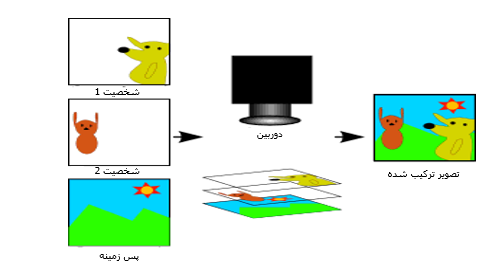
\includegraphics[width=\textwidth,height=\textheight,keepaspectratio]{Figures/Ch1/DifferentLayers.png}}

	\caption{لایه‌های مختلف}
	\label{fig:DifferentLayers}
\end{figure}

\section{پویانمایی کامپیوتری}

اگر بخواهیم نگاهی به تاریخچه‌ی انیمیشن‌های کامپیوتری بیاندازیم، مشاهده می‌کنیم که 
در حدود دهه‌ی 1980 میلادی شرکت دیزنی به عنوان یکی از اولین شرکت‌های جهان، شروع به 
دیجیتالی کردن خط لوله‌ی تولید پویانمایی سل‌ای خود کرد.
در این دیجیتال‌سازی بسیاری از روش‌ها و ایده‌‌های استفاده شده در پویانمایی سنتی،
به‌کار گرفته‌شد.
اولین مقالات این حوزه توسط آقای جان لستر از کارمندان پیکسار به عنوان 
"اصول پویانمایی سنتی به‌کار رفته در پویانمایی کامپیوتری سه‌بعدی"
ارائه شد.
در این مقاله اصول اولیه پویانمایی سنتی دوبعدی ترسیم شده با دست
و کاربرد آن‌ها در پویانمایی کامپیوتری سه‌بعدی شرح داده شده است.

پویانمایی کامپیوتری تنها محدود به دنیای سینما و فیلم‌های پویانمایی شده، نمی‌شوند بلکه به دنیای
بازی‌های کامپیوتری نیز ورود پیدا کرده‌اند. بازی‌های کامپیوتری سعی می‌کنند دنیای میان تماشاگران و فیلم را بشکنند و 
با تعاملی بودن و دادن آزادی عمل به بازیکن، سعی می‌کنند داستان را به گونه‌ای تعریف کنند که گویی بازیکن یکی از شخصیت‌های اصلی داستان است.
پویانمایی در بازی‌های کامپیوتری اهمیت بسیار بالایی دارد زیرا همانطور که گفته شد باعث 
جان بخشیدن به شخصیت‌ها می‌شود که اهمیت بسیار بالایی برای جلب توجه بازیکنان در هنگام داستان‌سرایی دارد.

با پیشرفت تکنولوژی همراه با استفاده از روش‌های گذشته، روش‌های جدیدتری برای تولید پویانمایی توسعه یافته‌است که 
در ادامه به چند مورد از آن‌‌ها می‌پردازیم.

\subsection{فریم‌های کلیدی و درمیان}

همانطور که اشاره شد در پویانمایی کامپیوتری از روش‌های موجود در 
پویانمایی سنتی استفاده شده است. در اینجا نیز فریم‌های کلیدی 
یک حرکت توسط پویانماها به وجود می‌‌آیند ولی فریم‌های میانی به جای اینکه توسط پویانماها به وجود آید،
توسط کامپیوتر با استفاده از روش های درون‌یابی به وجود می‌آیند.

\subsection{رویه}

در این روش، حرکت بر اساس یک الگوریتم بیان می‌شود.
درواقع انیمیشن‌ها در این نوع پویانمایی، توابعی با تعداد کمی از متغیر‌ها هستند.
به عنوان مثال یک تابعی را درنظر بگیرید که به گرفتن ورودی ثانیه، دقیقه و ساعت، 
یک شئ ساعت را خروجی دهد که عقربه‌هایش در جای مناسب با توجه به ورودی‌ها قرار گرفته باشد.
حال می‌توان با تغییر ورودی‌ها حرکت ساعت را شبیه‌سازی کنیم.

\subsection{مبتنی بر فیزیک}

پویانمایی مبتنی بر فیزیک پلی میان دنیای پویانمایی با 
دنیای واقعی است. در این روش با نسبت دادن ویژگی‌های فیزیک به اشیاء سه‌بعدی و سپس حل‌کردن
فرمول‌های فیزیک مانند فرمول حرکت یا فرمول‌های نیوتن،
فیزیک را شبیه سازی می‌کند.
پویانمایی‌های مبتنی بر فیزیک شخصیت را قادر می‌سازد تا حرکت‌های خود را 
به صورت پویا با محیط تنظیم کند.




\section{موتور بازی‌سازی}
موتور‌های بازی‌سازی پلتفرم‌هایی هستند که ساخت بازی‌های رایانه‌ای را آسان‌تر می‌کنند.
آن ها به شما این امکان را می‌دهند تا عناصر بازی مانند انیمیشن، تعامل با کاربر یا تشخیص برخورد میان اشیاء را در یک واحد ادغام و ترکیب کنید.
\cite{barczak2019comparative}
زمانی که از اصطلاح موتور بازی‌سازی استفاده می‌کنیم منظورمان نرم‌افزارهای قابل توسعه‌ای هستند که می توانند پایه و اساس بسیاری از بازی‌های مختلف باشند.
\cite{GameEngineArchitecture}
موتورهای بازی‌سازی متشکل از اجزای مختلفی هستند که قابلیت‌های لازم برای ساخت بازی را فراهم می‌کنند.
رایج ترین اجزای موتور بازی عبارتند از:
\cite{barczak2019comparative}
\begin{itemize}
    \item[-] مولفه‌ی صدا: نقش اصلی این مولفه تولید جلوه‌های صوتی در بازی است.
    \item[-] موتور رندر: وظیفه اصلی این مولفه تبدیل داده‌های ورودی به پیکسل‌ها، برای به تصویر کشاندن بر روی صفحه است.
    \item[-] مولفه هوش مصنوعی: این مولفه مسئولیت ارائه‌ی تکنیک‌هایی برای تعریف قوانین رفتار شخصیت‌هایی را دارد که توسط بازیکنان کنترل نمی‌شوند.
    \item[-] مولفه انیمیشن: نقش اصلی این مولفه اجرای انیمیشن‌های مختلف مانند حرکت است.
    \item[-] مولفه شبکه: وظیفه اصلی این مولفه قادرساختنِ بازیِ همزمانِ بازیکنان با یکدیگر، از طریق استفاده از دستگاه‌های متصل به اینترنت است.
    \item[-] مولفه منطق یا مکانیک بازی: این مولفه قوانین حاکم بر دنیای مجازی، ویژگی‌های شخصیت‌های بازیکنان، هوش مصنوعی و اشیاء موجود در دنیای مجازی و همچنین وظایف و اهداف بازیکنان را تعریف می‌کند.
    \item[-] ابزارهای نرم‌افزاری: وظیفه اصلی این ابزارها افزایش راندمان و سرعت تولید بازی با موتور بازی‌سازی است. آن‌ها توانایی اضافه‌کردن بسیاری از عناصر مختلف را به بازی‌ها، از انیمیشن و جلوه‌های صوتی گرفته تا الگوریتم‌های هوش مصنوعی، را فراهم می‌کنند.   
\end{itemize}

\section {موتور بازی‌سازی آنریل}

اولین نسل موتور بازی‌سازی آنریل توسط تیم سوینی، بنیانگذار اپیک گیمز
\LTRfootnote {Epic Games}
،
توسعه یافت.
سویینی در سال 1995 شروع به نوشتن این موتور برای تولید بازی‌ تیراندازی اول شخصی به اسم غیرواقعی
\LTRfootnote{Unreal}
کرد.
نسخه‌‌ی دوم موتور بازی‌سازی آنریل در سال 2002 منتشر شد. نسخه سوم نیز در سال 2004 پس از اینکه حدود 18 ماه در حال توسعه بود منتشر شد.
در این نسخه، معماری پایه‌ای موجود در نسخه‌ی اول مانند طراحی شی‌گرا، اسکریپت‌نویسی مبتنی بر داده و رویکرد نسبتا ماژولار نسبت به زیرسیستم‌ها وجود داشت.
اما برخلاف نسخه دوم که از یک خط لوله با عملکرد ثابت
\LTRfootnote{fixed-function pipeline}
استفاده می‌کرد، این نسخه به صورتی طراحی شده بود تا بتوان قسمت‌های سایه‌زنی سخت‌افزاری
\LTRfootnote{shader hardware}
را برنامه‌نویسی کرد.

موتور بازی‌سازی آنریل 4 در سال 2014 در کنفرانس توسعه‌دهندگان بازی
\LTRfootnote{GDC}
منتشر شد.
این نسخه با طرح کسب‌و‌کار اشتراکی برای توسعه‌دهندگان در دسترس قرار گرفت. این اشتراک به صورت ماهانه، با پرداخت 19 دلار آمریکا به توسعه‌دهندگان این اجازه را می‌داد تا به نسخه‌ی کامل موتور، از جمله کد منبع 
\lr {C++}
آن
دسترسی پیدا‌ کنند.
البته در سال 2015 اپیک گیمز موتور بازی‌سازی آنریل را به صورت رایگان برای همگان منتشر ساخت.
آخرین نسخه آنریل به اسم موتور بازی‌سازی آنریل 5 در سال 2020 معرفی شد. این نسخه از تمام سیستم‌های موجود از جمله کنسول‌های نسل بعدی پلی‌استیشن 5
\LTRfootnote{PlayStation 5}
و ایکس‌باکس سری 
\lr{X/S}
\LTRfootnote{Xbox Series X/S}
پشتیبانی می کند.
کار بر روی این موتور حدود دو سال قبل از معرفی آن شروع شده بود. در سال 2021 نسخه‌ای از آن به صورت دسترسی اولیه منتشر شد. به طور رسمی در سال 2022 نسخه‌ی کامل این موتور برای توسعه‌دهندگان انتشار یافت.
\cite{UnrealEngineWikiPedia}

\section{انیمیشن‌های کامپیوتری}
